\documentclass[a4paper,12pt]{article}
\usepackage[bahasa]{babel}
\usepackage{graphicx}
\usepackage{multirow}
\usepackage{enumitem}
\usepackage{listings}
\graphicspath{ {./img/} }
\begin{document}
\title{Laporan Praktikum Statistika Pertemuan 8}
%\author{Aldzikri Dwijayanto Prathama \\ {\small 195410189}}
\author{Aldzikri Dwijayanto Prathama 
	\\195410189}
\makeatletter
\begin{titlepage}
	\begin{center}
		{\huge \bfseries \@title }\\[14ex]
		
\includegraphics[scale=.8]{logo}\\[4ex]
		{\large \@author}\\[20ex]
		{\large \bfseries {SEKOLAH TINGGI MANAJEMEN INFORMATIKA DAN KOMPUTER
				AKAKOM YOGYAKARTA}}
	\end{center}


%{\large \@date} 
\end{titlepage}
\makeatother
%\maketitle
\newpage
\tableofcontents
\newpage
\section{Tujuan}
\begin{enumerate}
	\item Praktikan mampu menyajikan deskripsi nilai pusat 
	\item Praktikan mampu menyajikan deskripsi nilai dispersi
\end{enumerate}
\section{Dasar Teori}
\begin{enumerate}[label={\bfseries \Alph*.}]
	\item {\bfseries NILAI  PEMUSATAN}
	\paragraph{}
	Salah satu aspek yang paling penting untuk menggambarkan distribusi data adalah nilai pusat data pengamatan (Central Tendency). Setiap pengukuran aritmatika yang ditujukan untuk menggambarkan suatu nilai yang mewakili nilai pusat atau nilai sentral dari sekelompok  data (himpunan pengamatan) dikenal sebagai \textbf{ukuran pemusatan data (tendensi sentral)}.\\
	Ukuran nilai pusat/tendensi sentral (average) merupakan nilai pewakil dari suatu distribusi data, sehingga harus memiliki sifat-sifat berikut:
	\begin{itemize}
		\item Harus mempertimbangkan semua gugus data
		\item Tidak boleh terpengaruh oleh nilai-nilai ekstrim.
		\item Harus stabil dari sampel ke sampel.
		\item Harus mampu digunakan untuk analisis statistik lebih lanjut.
	
	\end{itemize}
	Terdapat tiga ukuran pemusatan data yang sering digunakan, yaitu:
	\begin{enumerate}[label=\alph*.]
		\item Mean (Rata-rata hitung/rata-rata aritmetika)
		\item Median
		\item Modus
	\end{enumerate}
%	\paragraph{Mean (arithmetic mean)\\}
%	Rata-rata hitung atau arithmetic mean atau sering disebut dengan istilah mean saja merupakan metode yang paling banyak digunakan untuk menggambarkan ukuran tendensi sentral. Mean dihitung dengan menjumlahkan semua nilai data pengamatan kemudian dibagi dengan banyaknya data. Definisi tersebut dapat di nyatakan dengan persamaan berikut:\\
%	\[\overline{x}=\frac{x{1}+x_{2}+x_{3}+x_{4}+....+x_{n}}{n}=\frac{\sum \limits_{i=1}^{n}x_{i}}{n}\]
	\item {\bfseries NILAI DISPERSI}
	\paragraph{}
	Ukuran  dispersi  atau  ukuran  variasi  adalah  ukuran  yang  menyatakan  seberapa  jauh nilai data  yang  berbeda  dari  nilai  pusatnya . Ukuran  dispersi  pada   dasarnya  merupakan  pelengkap  dari  ukuran  pusat  dalam menggambarkan  sekumpulan  data.  Dengan  ukuran  dispersi,  penggambaran  data  akan  lebih tepat dan jelas.
	Fungsi ukuran dispersi:
	Menunjukkan tinggi rendahnya penimpangan antar data.
	Mengeahui derajat perbedaan antar data\\
	{\bfseries Jenis Ukuran Disperse}
	\begin{enumerate}
		\item Jangkauan (Range, R)
		\item Variansi
		\item Simpangan Baku (Standar Deviasi) 
	\end{enumerate}
	
\end{enumerate}

\section{Praktik}
\subsection{Praktik 1}
\begin{center}
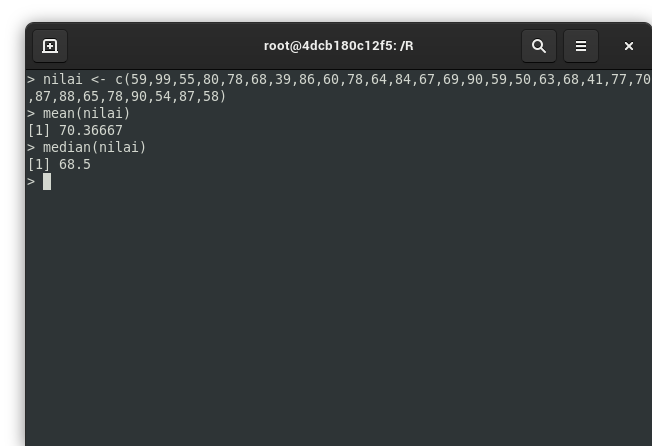
\includegraphics[scale=.6]{praktik01}
\end{center}
\paragraph{Pembahasan\\}
Pertama masukkan hasi nilai hasil ujian matematika dari 30 siswa ke variabel nilai dengan fungsi c, dengan perintah:\\
\texttt{nilai <- c(59,99,55,80,78,68,39,86,60,78,64,84,67,69,90,59,50,63
	,68,41,77,70,87,88,65,78,90,54,87,58)}\\
untuk menampilkan rata-rata dari data didalam variabel nilai gunakan fungsi mean:\\
\texttt{mean(nilai)}\\
Sedangkan untuk median gunakan fungsi median\\
\texttt{median(nilai)}\\
Dari output di atas dapat diketahui nilai ringkasan numeriknya, yaitu rata-rata nilai  adalah 70,36667 sedangkan nilai mediannya adalah 68,5.

\subsection{Praktik 2}
\begin{center}
	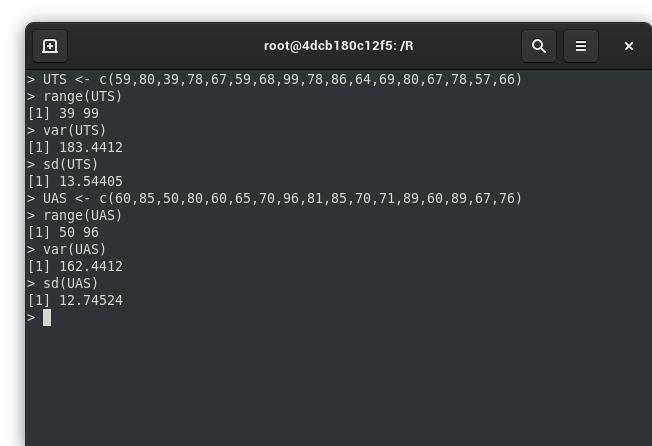
\includegraphics[scale=.6]{praktik02}
\end{center}
\paragraph{Pembahasan\\}
Masukkan data ke variabel UTS\\
\texttt{UTS <- c(59,80,39,78,67,59,68,99,78,86,64,69,80,67,78,57,66)}
Tentukan range dari data di variabel UTS\\
\texttt{range(uts)}\\
Untuk menentukan variansi data di variabel UTS gunakan\\
\texttt{var(UTS)}\\
Untuk menentukan standar deviansi dari nilai UTS\\
\texttt{sd(UTS)}

Masukkan data ke variabel UAS\\
\texttt{UAS <- c(60,85,50,80,60,65,70,96,81,85,70,71,89,60,89,67,76)}
Tentukan range dari data di variabel UAS\\
\texttt{range(UAS)}\\
Untuk menentukan variansi data di variabel UAS gunakan\\
\texttt{var(UAS)}\\
Untuk menentukan standar deviansi dari nilai UAS\\
\texttt{sd(UAS)}\\

Dari output di atas dapat diketahui nilai ringkasan numeriknya, yaitu  nilai range untuk UTS adalah 99 – 39 = 60, nilai variansi UTS nya  183,4412 , nilai simpangan baku untuk UTS adalah 13,54405.\\
Nilai range untuk UAS adalah 96 – 50 = 46, nilai variansi UTS nya  162,4412 , nilai simpangan baku untuk UTS adalah 12,74524.

\section{Latihan}
\subsection{Latihan 1}
\paragraph{Masalah\\}
Berikut ini data panen ikan di 20 kolam (kg):\\
40, 35,46,51,46,32,45,37,39,40,
42, 35,50,46,48,42,44,39,36,38,
56,43,54,36,36,38,42,45,38,40,
51,34,51,39,42,41,45,47,52,49\\
Tentukan nilai rata-rata, median, jangkauan, variansi dan simpangan baku dari hasil panen ikan teresbut.


\paragraph{Penyelesaian}
\begin{center}
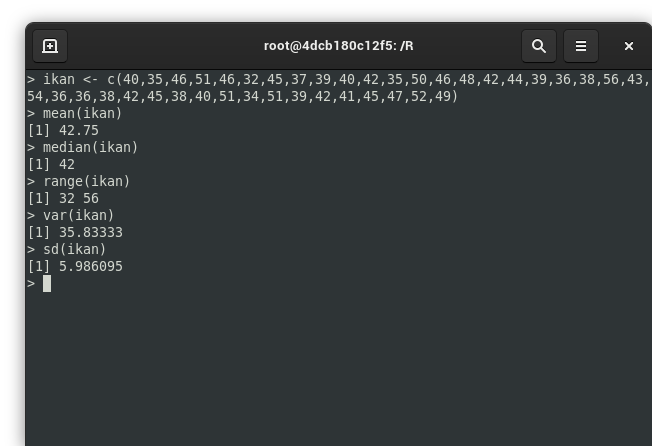
\includegraphics[scale=.6]{latihan01}
\end{center}
Masukkan data panen ikan ke variabel ikan:\\
\texttt{ikan <- c(40,35,46,51,46,32,45,37,39,40,42,35,50,46,48,42,44,39
	\\,36,38,56,43,54,36,36,38,42,45,38,40,51,34,51,39,42,41,45,47,52,49)}\\
Gunakan fungsi mean untuk mencari rata-rata dari data di variabel ikan:\\
\texttt{mean(ikan)}\\
Mencari median variabel ikan dengan fungsi median:\\
\texttt{medain(ikan)}
Tentukan range dari data di variabel ikan\\
\texttt{range(ikan)}\\
Untuk menentukan variansi data di variabel ikan gunakan\\
\texttt{var(ikan)}\\
Untuk menentukan simpangan baku dari variabel ikan\\
\texttt{sd(ikan)}\\
Dari output di atas dapat diketahui nilai ringkasan numeriknya, yaitu rata-rata hasil panen adalah 42,75 sedangkan nilai mediannya adalah 42. nilai range untuk data hasil panen adalah 56 – 32 = 24, nilai variansi data hasil panen adalah  35,83333 , nilai simpangan baku untuk data hasil panen adalah 5,986095.\\

\subsection{Latihan 2}

\paragraph{Masalah\\}
Berikut adalah data berat badan mahasiswa di prodi  Akutansi
\begin{table}[!ht]

	\begin{tabular}{|l|l|}
		\hline
		
		Pria & Wanita \\ \hline
		58 & 48 \\ \hline
		69 & 53 \\ \hline
		75 & 48 \\ \hline
		68 & 52 \\ \hline
		60 & 46 \\ \hline
		80 & 50 \\ \hline
		74 & 61 \\ \hline
		64 & 46 \\ \hline
		65 & 50 \\ \hline
		
	\end{tabular}
\end{table}
Tentukan nilai nilai rata-rata, median, jangkauan, variansi dan simpangan baku dari berat badan mahasiswa diatas

\newpage
\paragraph{Penyelesaian}
\begin{center}
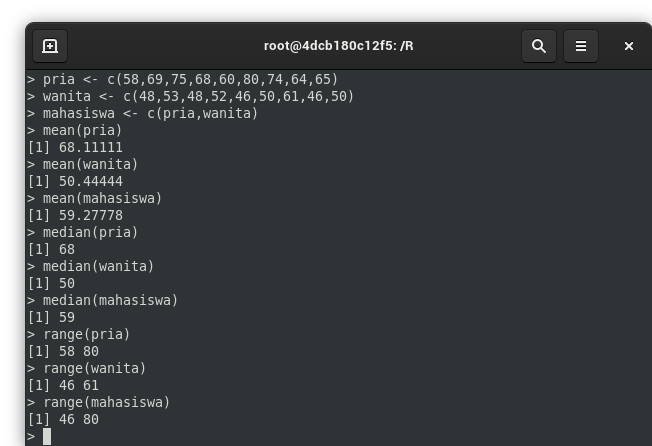
\includegraphics[scale=.6]{latihan02-1}
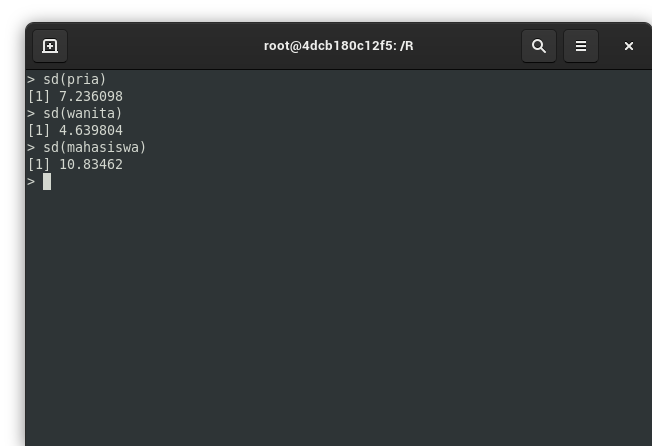
\includegraphics[scale=.6]{latihan02-2}
\end{center}
Masukkan data ke variabel pria, dan wanita, lalu buat variabel mahasiswa dengan data dari variabel pria dan wanita\\
\texttt{pria <- c(58,69,75,68,60,80,74,64,65)\\
wanita <- c(48,53,48,52,46,50,61,46,50)\\
mahasiswa <- c(pria,wanita)\\}
Dari output di atas dapat diketahui nilai ringkasan numeriknya, yaitu rata-rata berat badan pria adalah 68,11111, berat badan wanita 50.44444 , berat badan mahasiswa keseluruhan 57,27778. Sedangkan nilai mediannya berat badan pria adalah 68,  berat badan wanita 50, berat badan keselurahan mahasiswa 59. Nilai range untuk data berat badan pria adalah 58 - 80, berat badan wanita adalah46 - 61, berat badan mahasiswa keseluruhan adalah 46 - 80 .Nilai simpangan baku untuk berat badan pria adalah 7,236098, berat badan wanita adalah 4,639804, berat badan mahasiswa keseluruhan 10,83462.\\

\section{Tugas}
\paragraph{Masalah\\}
Berikut data berat badan sebelum dan sesudah melakukan dieti 15 mahasiswa :
\begin{table}[!ht]
	\begin{tabular}{|l|l|}
		\hline
		
		Sebelum & Sesudah \\ \hline
		59 & 40 \\ \hline
		80 & 80 \\ \hline
		59 & 50 \\ \hline
		78 & 80 \\ \hline
		60 & 60 \\ \hline
		69 & 65 \\ \hline
		68 & 60 \\ \hline
		99 & 96 \\ \hline
		78 & 81 \\ \hline
		86 & 85 \\ \hline
		64 & 60 \\ \hline
		69 & 71 \\ \hline
		50 & 44 \\ \hline
		57 & 54 \\ \hline
		65 & 60 \\ \hline
		
	\end{tabular}
\end{table}
Tentukan nilai , median, modus, mean range, variansi dan standar deviasi berat badan sebelum dan sesudah diet

\paragraph{Penyelesaian\\}
Karena dalam R tidak ada fungsi untuk menentukan modus, maka kita harus membuat fungsi modus sendiri
\begin{center}
	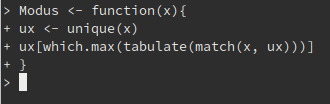
\includegraphics[scale=1]{fungsi}
	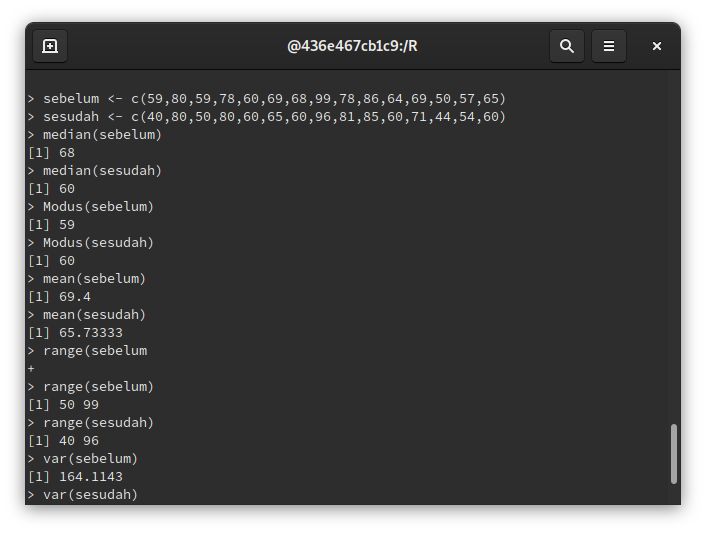
\includegraphics[scale=.6]{tugas1}
	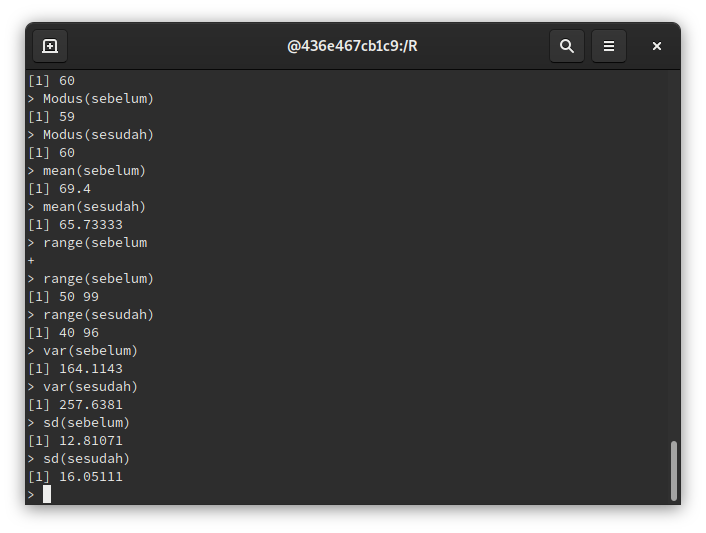
\includegraphics[scale=.6]{tugas2}
\end{center}
Dari output di atas dapat diketahui nilai ringkasan numeriknya, yaitu rata-rata berat badan sebelum diet adalah 69,4 , sesudah diet adalah 65,73333. sedangkan nilai mediannya sebelum diet adalah 68, sesudah diet adalah 60. Nilai range untuk data berat badan sebelum diet adalah 50-99, sesudah diet adalah 40-96, nilai variansi data berat badan sebelum diet adalah  164,1143, sesudah diet 257,6381, nilai simpangan baku untuk data sebelum diet adalah 12,81071 , sesduah diet adalah 16.05111. Sedangkan untuk modus data berat badan sebelum diet adalah 59, sesudah diet adalah 60.\\

\newpage

\section{Kesimpulan}
Mahasiwa mampu menyajikan deskripsi nilai pusat dan deskripsi nilai dispersi



\end{document}